%\addcontentsline{toc}{chapter}{Development Process}
\chapter{Development Process}



\section{Introduction}
%Introduce the specific model that you chose to use. 
% You need to describe briefly the life cycle model that you used. Do not force your project into the waterfall model if it is better described by prototyping or some other evolutionary model. You do not need to write about all of the different process models that you are aware of. Focus on the process model that you have used. It is possible that you needed to adapt an existing process model to suit your project; clearly identify what you used and how you adapted it for your needs.


The project used an evolutionary prototyping approach. There were two phases:
\begin{enumerate}
 \item requirements gathering; building the basic application structure, in particular submission of information; investigating appropriate technologies
 \item building the features from the initial feature list feature-by-feature; some were dropped due to difficulties with them or higher priority features - final list arrived at through this iterative process
\end{enumerate}

An Agile, iterative approach to the development of the software was initially chosen. It turned out that the approach did not fit the project / author / users context. In particular:

\begin{enumerate}
 \item The initial approach was actually not Agile to begin with (a problem of understanding what Agile actually entails).
 \item Agile requires a certain level of understanding of the technology (developer's side) and problem the software is solving (``customers''' or users' side).
\end{enumerate}

The length of the requirements gathering phase and the complexity of developing the most important features was initially underestimated. Analysis of the intermediate outputs and measurement against the initial aims suggested that a different scope was necessary. The new goals required a different approach, but that alone would not provide an answer as to what FundFind should have aimed for while remaining realistic.

Concentrating on and discussing the original goal of the FundFind project with interested parties proved fruitful. The overarching aims of ``learning about scholarly funding'' and ``prototyping a solution for sharing this information'' resulted in a leaner, more focussed set of requirements to work towards. Since work on the code had started and a basic web application was running, it was most appropriate to enhance this and peruse the chosen datastore's unique characteristics to add new features while retaining simplicity. This approach in the second phase of the project was essentially faster evolutionary prototyping (compared to the first phase), mostly due to building better understanding of the technologies involved and insufficient time to deliver all features on the list.

\subsection{Project management tools}
\label{pm-tools}
A project management piece of software suited for Agile approaches was chosen to manage this project and was used successfully throughout: PivotalTracker. The project's progress and a list of features (in priority order) has been publicly available at \cite{pm} throughout the project's current lifespan (October 2012 - April 2013).

A private source code version control repository was set up with GitHub \cite{github}. It is only private due to several concerns:
\begin{enumerate}
 \item The licensing status of the IDFind project which FundFind was forked off, was unclear. In fact, with no license statement anywhere in the repository, the default copyright rules apply and FundFind could not have been legally based on IDFind without explicit written permission from the authors. However, since IDFind's only contributors were Cottage Labs LLP and the author of FundFind, this did not delay FundFind's development. Nevertheless, IDFind's licensing status was not cleared up until April 2013.
 
 \item There were concerns about the quality of FundFind's code and the repository. GitHub is home to enough orphan repositories which are all almost empty or without proper licensing, either of which makes the project useless in terms of its Open Source aspect.
 
 \item It wasn't quite clear whether the code could be released during the official timeline of the final-year Major Project module at the author's institution. One of the main ideas in open-sourcing code is that others can contribute to it, but that would have significantly complicated matters in terms of reviewing the final version of the code. Cottage Labs LLP would like to contribute, but agreed that they are busy enough at the moment to look at the codebase after the 26th April 2013 (by which time a copy of FundFind's codebase would have been handed in).
\end{enumerate}

Furthermore, a private repository holding all of the other outputs of the author's Major Project (Outline Specification, Progress Report, presentation files, this document and so on) was set up purely for back-up purposes.

\section{Evolution of the Development Process}
Initially, Agile practices such as Pair Programming \cite{pairprg}, full Scrum \cite{Scrum} and Feature-Driven Development were deemed unsuitable since they are aimed at groups of developers. Behaviour-Driven Development (with Cucumber \cite{cucumber}) was considered, but requires more commitment from the users - they need to learn an English-like domain-specific language which describes how the system is going to behave which didn't sit well with assumption \#2 above and turned out to be the right decision as that assumption proved correct.

Thus, initially, with no methodology fitting the precise needs of the project and the Agile Manifesto \cite{agile-manifesto} in mind, a methodology of an Agile \emph{character} was planned, using the Extreme Programming lifecycle as a base \cite{xp-lifecycle}. The idea was to use ideas such as Release Planning (plan a set of features), Iteration (develop in small increments) and Stories (described above).

The basic steps which were defined were:
\begin{shadequote}
\begin{enumerate}
	\item Meet with a variety of potential users from the chosen user group (\S\ref{focus-groups}), trying to pick them so that each one has a different professional perspective on scholarship.
	\par\emph{Emanuil Tolev in FundFind Progress Report \cite{progress-report}}
	\setcounter{tmpc}{\theenumi}
\end{enumerate}
\end{shadequote}

This worked well, with candidate postgraduates, postgraduates, research assistants (post-doctoral), lecturers and developers all agreeing to give a bit of their time. The meetings were not as regular as initially hoped (1 per month with each user) due to users' commitments, author's committments and a particular characteristic of this project.

Looking at requirements presented in \S\ref{audience}, it is easy to see that the basic searching and sharing of opportunities were two \emph{really} important functions. Sharing is used to different ends by research officers, lecturers, postgraduates and funders, while searching is useful for different reasons to pretty much everybody. However, getting timely feedback from all target users was not considered to be possible - and that is required for iterative development. It was actually considered (and turned out to be - \S\ref{impl-hard-basics}) difficult enough to produce a prototype which made progress in satisfying the initial requirements of \emph{multiple} groups. Thus, meetings essentially happened at the start at the project (October, November, December) and at the end, in March and April, since most of the time inbetween was spent getting those two important features right. Advanced functionality was planned in March and developed in April and is described below in \S\ref{final-reqs}.

\begin{shadequote}
\begin{enumerate}
	\setcounter{enumi}{\thetmpc}
	\item Define \emph{and prioritise} the functionality of the project with each user in the form of the ``stories'' mentioned above. Record the results using the chosen project management tools (\S\ref{pm-tools}).
	\par\emph{Emanuil Tolev in FundFind Progress Report \cite{progress-report}}
	\setcounter{tmpc}{\theenumi}
\end{enumerate}
\end{shadequote}

%This turned out to be a really good idea 

\begin{shadequote}
\begin{enumerate}
	\setcounter{enumi}{\thetmpc}
	\item Release planning - prepare an initial timeline of which project features are to be released when and denote ``release points''. This work can be repeated as required - the order and the features themselves might change on the basis of user feedback over time (this is how Agile projects try to deliver more value by responding to changing requirements). The total size of the work and the size of each feature will most probably remain the same. This piece of work produces the ``Project Timeline'' and the current version is included in \S\ref{timeline}.
	\par\emph{Emanuil Tolev in FundFind Progress Report \cite{progress-report}}
	\setcounter{tmpc}{\theenumi}
\end{enumerate}
\end{shadequote}

\begin{shadequote}
\begin{enumerate}
	\setcounter{enumi}{\thetmpc}
	\item Iterate - every week is a self-contained unit of work consisting of coding, documentation and write-up work. Before starting to code each week, break up that week's story into tasks so goals can be tracked more effectively and there is something to be accomplished each day.
	\par\emph{Emanuil Tolev in FundFind Progress Report \cite{progress-report}}
	\setcounter{tmpc}{\theenumi}
\end{enumerate}
\end{shadequote}

\begin{shadequote}
\begin{enumerate}
	\setcounter{enumi}{\thetmpc}
	\item Repeat items 1 and 2 - meaning regular meetings with previously chosen users - one per user per month, demonstrate the latest features and record the feedback.
	\par\emph{Emanuil Tolev in FundFind Progress Report \cite{progress-report}}
	\setcounter{tmpc}{\theenumi}
\end{enumerate}
\end{shadequote}
	


% Within the coding part of each iteration, Test-Driven Development is employed using both unit and integration tests (the latter via browser automation with Selenium \cite{selenium}). This will be the evidence (on a basic technical level) for the ``correctness'' of the software. A basic form of Continuous Integration \cite{ci} will also be used - the Jenkins \cite{jenkins} software is currently being evaluated for the job. It basically runs all automated tests continuously, helping to detect regressions in code quality.
% 
% This methodology makes for a considerably simpler lifecycle than the Extreme Programming one (a visualisation of which can be accessed at \cite{xp-lifecycle}). This is intentional as there are only about 11 (potentially 13) weeks which allow for programming work as can be seen in \S\ref{timeline}.
% 
% The length of one iteration will be one week. Considering the tight deliverable deadlines (see \S\ref{timeline}), this will keep work on the project focused and will force the definition of user stories of a manageable size.

%Agile approaches usually \emph{avoid} defining ``size'' - how long it will take to implement a story. Rather the complexity of each story is estimated using \emph{arbitrary} numbers (some people prefer to use larger/smaller animals) - how difficult it is to implement that story relative to other stories. If a story seems too \emph{complex}, it needs to broken up. This project uses the Fibonacci number sequence \cite{fibonacci} and ``too complex'' is a complexity estimate of more than 3. Previous experience with the technologies involved has also helped provide a link between complexity and ``how much time will it take'', thus helping enforce a maximum of 1 week to complete a story and add value to the software.

% Saying ``actual features being implemented could change due to the Agile project development methodology'' as the Progress Report did does not make the approach Agile, as Agile is not a stick that one uses to prune excessive features at will - it is an approach that the developer sticks to.

\section{Modifications}
%Did you have to modify the model to suit a one-person project. If so, what did you change and why? 
In the Progress Report features were planned and \emph{scheduled} in a timeline before development took place, but that is \emph{not} the Agile way at all.

\subsection{What is Agile?}
Agile is about getting work done in an iterative fashion so that there is always working software for the users to use. Estimates in Agile are about effort, complexity and risk. Estimates are also \emph{relative} - when new features are added to the project scope, they are estimated in comparison to previously added ones. (For a commonly used estimation points scale and more elaboration on Agile estimation, see \cite{agile-estimate}.) If numeric points are used for the estimation, the project ends up with several hundred / thousand points worth of features.

Since those are prioritised by the customer/users, work can then start. What Agile teams seem to do is to essentially see how quickly they get through work - how many points they go through per week, which is called the ``velocity'' of the team.

Only then is it possible to estimate how long all of the initially requested features will take to develop - by taking into account their ``size'' (relative to each other) and the team's abilities. Taking the total project size and dividing it by the weekly velocity gives a rough idea of how many weeks it would take to complete all requested features. Let this be |time_required|.

If |time_available < time_required|, then the scope of the project simply has to be limited, i.e. features have to be dropped, and this only becomes clear once velocity is established (so at least a few weeks after development has started). In other words, however many features there \emph{turns out} to be time for in the development process are \emph{what gets done}, which is why there is so much emphasis on having the users involved - prioritising the functionality themselves.

\subsection{Is it Agile?}

FundFind's Progress Report \cite{progress-report} stated that an Agile-like methodology had been chosen - the main concept being user stories which allow capturing user requirements very quickly in an informal way.

Having a list of desirable features is great, having a schedule of which one will be delivered when - not so much. The point of Agile is taking the specifics of the development team and users' knowledge (and specificity of their desires) into account. A fully pre-defined plan - even one informed by meeting users, such as in this case - disregards all of this and does not conform to Agile's flexibility requirements. (Responding to change better than more conventional approaches is usually one of the first touted benefits of Agile approaches.) 

Figure \ref{fig:timeline} presents that initial plan.
\newpage
\begin{figure}[H]
\centering
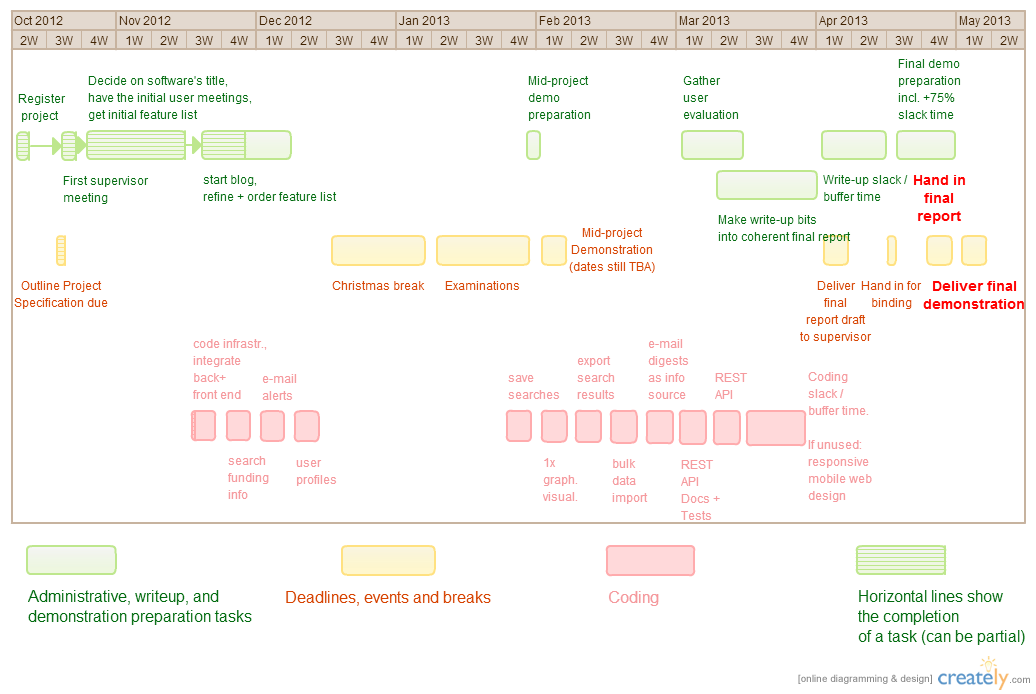
\includegraphics[height=0.6\textheight,angle=90]{Images/timeline.png}
\caption{FundFind initial timeline}
\label{fig:timeline}
\end{figure}
\newpage

\subsubsection{Underestimation}

The main reasons for choosing Agile were
\label{agile-reasons}
\begin{enumerate}
 \item Agile's perceived advantage in pinning down changing requirements.
 \item Less formal communication with the users, who are all busy professionals. It was assumed they would not have sufficient time for writing functional specifications, even in collaboration with the author (as can sometimes be assumed in industry).
 \item Linked to the user communication reason was a concept which many Agile methodologies used - user stories. These are short sentences (or rarely, paragraphs) which describe a single piece of functionality - a single ``thing'' that the user wants to do with the system.
\end{enumerate}

However, it turned out that both the complexity of the scholarly funding field and the author's ability to concretise fuzzy requirements, as well as their technical skill had been underestimated (elaborated upon in Chapter \ref{eval}). The fact that requirements had to be gathered and concretised is not unusual in Agile, but playing both developer and user was a problem. 

Neither did users have enough time to be properly involved throughout the project, nor did the author have enough domain knowledge to understand the requirements and develop quickly enough \emph{in order to get the users involved} in the way in which Agile understands involvement.

This conclusion and the process of arriving at it, ultimately, are the reason why the initial Agile-like development process was deemed unsuitable and why the project's progress is split so starkly into two phases as per Figure \ref{fig:new-process}.

The initial reasons for devising an Agile-like process (above) proved to (mostly) be steps in the right direction, however:
\begin{enumerate}
 \item The flexible requirements reason did not work out so well since it turned out the requirements did not change or need to change. Issues with funding data have been present for a while and a system which tries to prototype fixes through Open Data for some of them needs (a) developer(s) who know these issues inside out. of course, the requirements gathering can still be done in an Agile way, but needs to be mostly completed before development starts. Defining the problem, in this case, had to come before solving it.
 
 It could be argued that this was only a problem since the developer was also the ``initiator'' of the project (i.e. had to play user a lot more than usual). If a particular funder, Higher Education Institution or an organisation like the Open Knowledge Foundation wanted a project like this done, they would already know of certain problem characteristics - such as \emph{particular} drawbacks of having so much funding data ``closed''. Then, more targeted exploration could be done and technical development would also have more precise targets to meet.
 
 This is, in part, what caused the development process to look a lot more like \textbf{evolutionary prototyping} with a lot of requirements gathering between the prototype versions in Figure \ref{fig:new-process} rather than an Agile iterative approach.
 
 \item The assumption that users won't have time for anything but informal problem specification turned out to be correct. Thus, the ``stories'' concept proved to play an important role when gathering requirements from the target audience in short meetings, on the go or at hackdays.
 
 \item The project's stories have been publicly accessible at the PivotalTracker management tool continuously throughout the exploration phase of the project which was used to record the aforementioned informal requirements. The ``Icebox'' still contains the list of features as prioritised by the various users who have been consulted during the exploration phase.
\end{enumerate}

\section{Requirements}
\label{devprocess-requirements}
% In most cases, the agreed objectives or requirements will be the result of a compromise between what would ideally have been produced and what was felt to be possible in the time available. A discussion of the process of arriving at the final list is usually appropriate.

% not everything described in audience could be done

In this case, the project's requirements (in a suitable share-able form) are actually part of the expected project output, as one of the main aims is to learn about the scholarly funding field and identify needs.

\subsection{Requirements Gathering}
The process was essentially arranged 0.5h and 1h meetings with interested users and talking about

\begin{enumerate}
 \item what features they might find useful in a system such as FundFind and how the current list (as of the meeting) should be prioritised
 \item about the scholarly funding field in general (in an attempt to get everybody's point of view and be able to learn what their needs might be from the differences in the way people approached the field)
 \item about their role in this field (if any) in a further attempt to gather user needs information that might not have been otherwise articulated
\end{enumerate}

The results of each meeting fed into the next one due to item \#1. The final result is the list of requirements below.

It was quite difficult to get users to articulate what they need - FundFind does not match their current workflow, so there was a disconnect between the way they thought and the questions asked (e.g. ``saving searches'' means nothing to somebody who does not use a particular interface or system to search - it is akin to asking them if they save a copy of Google's results page for later use). This is the reason items \#2 and \#3 made it into the interview methods above after the first meeting.

Both of these methods required significant interpretation on the interviewer's side to produce useful results. While they certainly worked for generating new feature ideas, there wasn't much guarantee that those ideas would match the users' actual needs. Interpreting without much domain knowledge was one of the most difficult parts of the whole project.
% process - meetings etc.; any difficulties
% results - intermediary list - below

\subsection{Initial Requirements}
\label{initial-reqs}
The initial requirements were informed by the general needs of the various audience groups (\myref{audience}).

They are listed below alongside changes which were made (kept/dropped/changed/changed priority). Further discussion on the lessons learned and future work enabled by the dropped features is presented in \myref{future-work}. Features which went through major changes are discussed below in \myref{new-reqs}.

In \textbf{order of importance}:
\subsubsection{Search For Scholarly Funding Opportunities}
\begin{itemize}
 \item \textbf{Why}: It's the implementation of one of the main project goals - making funding information discoverable. Every single audience group needs it in one way or another.
 \item \textbf{Priority rationale}: All users decided it was a top-priority feature, very much the main point of a system like FundFind.
 \item \textbf{Decision}: \textbf{Kept as-is}. No information suggested that this had actually become any less important than when the project started, and although the project goals changed when it became clear how much expertise was needed to actually do everything well, this was still an important software feature.
\end{itemize}

\subsubsection{Submit Information About A Scholarly Funding Opportunity}
\begin{itemize}
 \item \textbf{Why}: In a similar vein to searching for such opportunities, multiple audience groups need it, albeit for different  reasons (a funder might want to make their opportunity more discoverable, while a PhD candidate can just share a good opportunity with their peers).
 \item \textbf{Priority rationale}: Core to the crowdsourcing functionality of the project. Actually incentivising users to do this is a different matter entirely. That is part of the point of FundFind though - through providing the capability to share, it gives a reference point to related conversations and feedback, (hopefully) allowing developers to understand why the various users do not want to share funding information.
 
 of course, this requires the search functionality to be present to provide great value to the project and is thus still second.
 \item \textbf{Decision}: \textbf{Kept as-is}, for the same reasons as the feature above.
 
\end{itemize}

\subsubsection{Submit Information About Funders}
\begin{itemize}
 \item \textbf{Why}: At the start of the project there were concerns that the various funding opportunities are vastly different in their purpose, format and thus, the data available about them. In order to alleviate this expected problem, this idea was presented to users and was found to be reasonable.
 
 In essence, if the funding opportunity data isn't good enough, a catalogue of funders would still be quite valuable. It was presumed to include some information to let the user search for an appropriate funder - like tagging the funders, or describing their interests.
 
 The idea actually came from a different Open Knowledge-related project called ACat (\textbf{A}cademic \textbf{Cat}alogue) \cite{acat} - an attempt to mine all information on all academic publishers, their journals \emph{and articles}. Even though ACat was just a hackday idea and hasn't evolved much since June 2012, it clearly showed the importance and value of having a list as simple as ``all UK academic publishers''.
 
 \item \textbf{Priority rationale}: Similar reasons to the feature above for this one to be so high up in the list in terms of crowdsourcing functionality. Its importance is very much tied to submitting information on funding opportunities - the more difficult it is to reconcile data from multiple sources (within the current scope), the more important this becomes.
 \item \textbf{Decision}: \textbf{Kept as-is}, for the same reasons as the feature above.
\end{itemize}

\subsubsection{Create Profiles}
\begin{itemize}
 \item \textbf{Why}: Submissions of data could not be anonymous \emph{to the system} - the submitter has to be authenticated and logged in some way, otherwise the submission forms will likely become the target of spam bots. It also helps with data quality, although admittedly on a very basic level - essentially, if a user is bothered to register, they are less likely to submit random junk into the system.
 
 This feature could include more than a username and a password however - it could include declaring research interest keywords and affiliations (the latter having been recorded as a separate feature at user meetings - see below).
 \item \textbf{Priority rationale}: Really desirable to enhance the basic functionality described above, but not as vital as actually having said functionality work in the first place.
 
 Other features which did not fit in the initial timeline at all but were earmarked for inclusion into a ``Future work'' section also require this (for example, research officers' reports \myref{future-research-officers-reports}).
 \item \textbf{Decision}: \textbf{Kept. Not much changed} except ``could include more than username and password'' became ``includes more...'' as no particular difficulties arose during the design or implementation of these additional fields.
\end{itemize}

\subsubsection{Visualise Data}
\begin{itemize}
 \item \textbf{Why}: It was thought that the Analyst audience group \myref{audience-analysis} would have an interest in this as it might spark other ideas about visualising funding data. Furthermore, scholars themselves might have had use for the result of the analysis - such as knowing how much their field is being funded at the moment.
 \item \textbf{Priority rationale}: Showcased the benefits of opening up funding data, which is one of FundFind's goals.
 \item \textbf{Decision}: \textbf{Dropped}. This turned out to be a little ill-defined. It embodied the quintessential software development problem of trying to predict what users want without actually knowing or being able to venture a good guess. The initial reasons as to why a visualisation might be useful are still true, of course, but it turned out developers who had done other Higher Education work understood the benefits of visualising such data quite well. Similarly, scholars could tell how well their field was funded just by looking at the data - the problem being that creating a visualisation that hid data appropriately and thus decreased cognitive load or increased insight was actually quite difficult. Representing the data in some much simpler visual way was not as hard, but also far from useful for people used to interpreting textual and numeric data. These insights were gained mainly during the Gateway to Research hackday (\myref{audience-analyst}).
\end{itemize}

\subsubsection{E-mail Alerts}
\begin{itemize}
 \item \textbf{Why}: Requirements gathering showed users using e-mail alerts / digests to receive the newest calls from funders. Thus, FundFind should probably offer a similar service as it federates such information.
 \item \textbf{Priority rationale}: Simply get users to use FundFind. With it, they would be getting the same information they could elsewhere, so this is just covering for value proposition \#2 from \myref{value-propositions}.
 \item \textbf{Decision}: \textbf{Dropped}. Turned out data - getting data - was more important than the gimmicks of managing data. This is where FundFind's role as a prototype and a limited vehicle of learning came into play.
\end{itemize}

\subsubsection{Saving Searches}
\label{reqs-saving-searches}
\begin{itemize}
 \item \textbf{Why}: In a similar fashion to e-mail alerts, this was thought to be important as it allowed for better management of data and reduced repeated search effort.
 \item \textbf{Priority rationale}: Part of value proposition \#3 - additional features. Other features such as e-mail alerts actually could be implemented more easily after this one is done - however, users did not think it was such a high priority. It also turned out that searches can already be shared just by copy/pasting the URL of the search page (\myref{impl-facetview}.
 \item \textbf{Decision}: \textbf{Dropped}. Similarly to e-mail alerts, it turned out data is the first thing to get into the application and leave enhancements for later.
\end{itemize}

\subsubsection{Harvesting Funding Data From E-mail Digests}
\label{devprocess-feats-email-harvest}
\begin{itemize}
 \item \textbf{Why}: This is one of the features which actually deal with importing data, fulfilling part of FundFind's core mission of federating funding data.
 \item \textbf{Priority rationale}: The importance of this was downplayed by the author - users did not have much to say on it, since they did not particularly care for the details of how FundFind was going to get its data, as long as it had some and they could use it.
 \item \textbf{Decision}: \textbf{Changed}. This is a good idea - however, all the information turned out to be available in machine readable formats (for the funders which were considered). It was also technically quite challenging (\myref{impl-email-parse}).
\end{itemize}

\subsubsection{Tagging Research as "Potentially of Interest to" Users and Groups}
\begin{itemize}
 \item \textbf{Why}: Part of showcasing the benefits of opening up and sharing funding data - enables scholars and research development officers to target the sharing of opportunities. May also enable funder representatives to target their funding calls better, although care has to be taken since the two sides of the ``advertisement'' may well have different goals.
 \item \textbf{Priority rationale}: This is a nice feature, but builds on profiles, search and submissions working, so just has to be done after them.
 \item \textbf{Decision}: \textbf{Kept as-is}.
\end{itemize}

\subsubsection{Specify Affiliation and Interests}
\begin{itemize}
 \item \textbf{Why}: This is actually the ``other end'' of tagging research - specifying where the user works (institution, research group, country) and what field the user works in (interests) enables the usage of the tags associated with research data.
 \item \textbf{Priority rationale}: Similarly to tagging research, this feature builds on everything before it, clearly part of value proposition \#3.
 \item \textbf{Decision}: \textbf{Kept as-is}.
\end{itemize}

All initial features described below were lower priority or in some way optional in relation to the main aims of the project.

\subsubsection{Responsive Mobile Web Design}
\begin{itemize}
 \item \textbf{Why}: FundFind is all about sharing data, thus it made sense to let people share in as many contexts as possible. The Design Rationale \myref{design-rationale} elaborates further on this feature, which is actually a UI design characteristic. It was also of personal technical interest to the author - responsive web user interfaces are everywhere in the Open Knowledge field. Some work better, some worse, yet one thing is clear - learning how to develop them is important. Preliminary research also showed that implementation might not actually be that difficult (\myref{impl-mobile}), especially with a more lax testing strategy (\myref{testing-mobile}).
 \item \textbf{Priority rationale}: As technically nice as this is, it was certainly not prioritised highly by users. Therefore, it was given a lower priority than the main functions of the application.
 \item \textbf{Decision}: \textbf{Kept as-is}.
\end{itemize}

\subsubsection{Bulk Funding Opportunity Data Import}
\begin{itemize}
 \item \textbf{Why}: Importing funding information records one-by-one can get quite boring, time-consuming and tiring - all the characteristics of a task that is ready to be automated. This was mainly conceived as a feature for the Analyst audience group (\myref{audience-analyst}), specifically more advanced users who might want to use the software itself and load it up with data they are interested in - not the data all other users have shared on the public FundFind instance. This also includes potential contributors to the code. Another potential target was funder representatives, who may have access to funding opportunity information from their organisation in a structured format and would rather just upload it than copy/paste the records one-by-one.
 \item \textbf{Priority rationale}: This feature has quite a narrow focus - a (very) narrow subset of the audience of the project.
 \item \textbf{Decision}: \textbf{Dropped} - it was just really of very limited use. Even backing up the data in the public FundFind instance does not require this feature, as the datastore can be backed up with a simple file copy command (\myref{design-datastore}).
\end{itemize}

\subsubsection{Harvesting Historical Funding Information}
\label{devprocess-feats-harvesting-historical-info}
\begin{itemize}
 \item \textbf{Why}: Historic funding information can be quite valuable since it can grant insight into what was previously funded. If this includes the most recent 1-10 years of data, it could be used to see how fields develop. While hopefully no scholar would choose their field based solely on its history of funding, they could see how to pitch their work most effectively - often, it is difficult to strictly categorise research.
 
 Something which came up during meetings was the fact that helping gain such insights from historical data might be just as, and sometimes more, helpful to \emph{obtaining} funding than just the sheer ability to \emph{find} it more easily.
 \item \textbf{Priority rationale}: FundFind had to focus on current funding opportunities.
 \item \textbf{Decision}: \textbf{Dropped}.
\end{itemize}

\subsubsection{RESTful API}
\begin{itemize}
 \item \textbf{Why}: Allow integration with other Open Knowledge projects, also vital to being able to consider FundFind an Open Knowledge project. If data is being federated from multiple sources, then it better be exposed in some way. The Design Rationale \myref{design-rationale} elaborates further on this feature.
 \item \textbf{Priority rationale}: Targets only the Analyst audience group (\myref{audience-analyst}).
 \item \textbf{Decision}: \textbf{Kept as-is}.
\end{itemize}

\subsubsection{Exporting The Results of Searches}
\begin{itemize}
 \item \textbf{Why}: Simple convenience - being able to save a list of relevant funding opportunities for later perusal.
 \item \textbf{Priority rationale}: Everything else has some function beyond pure convenience and this would not save that much time or effort in any case. Similar to saving searches (\myref{reqs-saving-searches}), searches can already be shared via the search page URL (\myref{impl-facetview}) which further reduced the priority of this feature, since the same search should yield quite similar results (based on the assumption that a search worth saving is a pretty specific search). This was also consistently rated as low priority in user meetings.
 \item \textbf{Decision}: \textbf{Dropped}. It is hard enough to find \emph{one} highly relevant funding opportunity - finding multiple ones is not something that will happen easily without getting quite a lot of data into FundFind.
\end{itemize}

\subsection{New Requirements}
\label{new-reqs}
A number of new features were inserted into the initial list during development - mostly stemming from new knowledge about related projects and data, or what was technically feasible.

\subsubsection{Harvest Funding Data From Machine-Readable Sources}
\begin{itemize}
 \item \textbf{Why}: It is far easier to process RSS feeds such as the EPSRC Open Calls RSS Feed \cite{epsrc-rss} than it was to process the EPSRC Funding Call E-mail Alerts, as discussed in \myref{impl-email-parse}.
 \item \textbf{Priority}: Replaced \myref{devprocess-feats-email-harvest}.
\end{itemize}

\subsubsection{Suggesting Relevant Historical Data}
\begin{itemize}
 \item \textbf{Why}: As discussed in \myref{devprocess-feats-harvesting-historical-info} above, it was discovered that this is actually a good way to achieve the end goal of funding scholarship. This project may have started as being about discovering \emph{current} funding information, but this itself stemmed from the overarching goal getting more funds to more scholars. This only became possible quite late in the development process as Gateway to Research's data was discovered by the author in March and gave a concrete foundation on which to build this feature.
 \item \textbf{Priority}: Lowest, tacked onto the end of the feature list. Very experimental due to potential data issues, lack of discussion with actual scholars (only other developers) and lack of clarity around presenting the information on the user interface. It was also technically quite ill-defined and difficult to achieve.
\end{itemize}

\subsection{Final Requirements}
\label{final-reqs}

%REPEATS INFO FROM NEW REQUIREMENTS SECTION ABOVE The advanced functions themselves were also not just requirements which were further down the requirements list (such as RSS and E-mail harvesting of data), but were driven by what was possible - mostly in terms of skill and data availability, both of which played a big role throughout the project. The Gateway to Research project hackday (see \myref{audience-analyst}) finally gave concrete enough insight and a large historical data source of funding data which could, together, be used to produce a new feature.

% just list the pruned list, nothing else to say about these after the Decision items above
\begin{enumerate}
\item Search For Scholarly Funding Opportunities
\item Submit Information About A Scholarly Funding Opportunity
\item Submit Information About Funders
\item Create Profiles
\item Harvest Funding Data From Machine-Readable Sources
\item Tagging Research as "Potentially of Interest to" Users and Groups
\item Specify Affiliation and Interests
\item Responsive Mobile Web Design
\item RESTful API
\item Suggesting Relevant Historical Data
\end{enumerate}


% TODO REVIEW where to put this. You should briefly describe the design method you used and any support tools that you used. You should discuss your choice of implementation tools - programming language, compilers, database management system, program development environment, etc.

\section{Design Process}
%TODO fill in!
% briefly describe the design method you used and any support tools that you used
% context and process implications on design

%TODO write this after the overview diagram in the first section is done

\section{Techologies used}
\label{devprocess-tech-used}
% TODO REVIEW careful about point of view - this is about the development process and how the tools used impacted it.
% ah screw it, just write reasons, can cut words later.

% context and process implications on implementation tools
% programming language, compilers
% database management system
% program development environment
% etc.
% frameworks
% always looking at other people's code, other FLOSS projects within OK movement
% bootstrapping the codebase from IDFind
% bootstrapping data gathering from bibserver

As \myref{existing-works} and \myref{design-rationale} point out, Python was chosen as the main programming language of the application. HTML5, CSS and Javascript were used for the user interface. Similarly to the Python choice, this was due to multiple other Open Knowledge projects using them in this manner - so it would be easy for interested developers to read the code and contribute. Previous personal experience with these technologies helped as well, as this is a sole developer project.

%Python is not without its faults, of course. Despite trying to be very newbie-friendly, the import system is difficult to understand, and the problem continues as users move on to intermediate proficiency as well. Understanding more advanced issues seems to be difficult even when its initial challenges have been mastered. The point is easily illustrated by the number of questions related to ``python import'' on the popular programming Q$+$A site stackoverflow.com \cite{so-python-import}, especially if the number of duplicates is considered.

%This isn't just a problem for reusing code, it is a problem for organising code in an application. At least 6-7 hours had to be spent in order to understand how to do something as (expectedly) simple as importing other modules within the same application, and why seemingly unrelated (or even \emph{no}) changes seemed to result in an entirely unrunnable project.

Basing the main application on another project that the author had participated in meant that a great deal of bootstrapping time was saved. A lot of knowledge about using the underlying Python frameworks was also reused. This was also partially true when the FundFind data harvester was written as it was again based on another Open Knowledge project, but the author had no previous experience with that code.

On the other hand, trying to create something to the standards enforced by other projects in the same context (Open Knowledge) forced quite a lot of reading that might not have been strictly necessary outside this context.

Python's interactive (REPL - Read, Evaluate, Print, Loop) interpreter was of great help to the development process. Instead of having to write a program in a file and then run it, the developer can type out the rough sequence of commands they want and see the results immediately. Seeing the results of a \emph{previous} command can be very important if the developer does not know or has just forgotten exactly what its output will be or look like. If the interpreter is run in the project's directory, all modules and other existing project bits can be accessed in the same way as in a written script.

Python's philosophy of readability (no semicolons, indentation matters, new line means new statement) and certain programming conventions which have been built up around it meant that the parent codebase was quite easy to understand.

Previous experience combined with the usage of relevant libraries meant that the quirks in developing with HTML and CSS - mainly the way CSS applies to HTML elements - did not delay development. On the other hand, having to learn how to work with the libraries certainly took some extra time, but saved a lot more (\myref{impl-ui}).

The RESTful JSON API that the chosen datastore (elasticsearch) provides also accelerated the process somewhat, since the all of the project's data could be retrieved by pointing a web browser at
\\ |http://localhost:9200/fundfind/_search?q=*|.

The command-line \textbf{V}i \textbf{IM}proved (vim) editor was used in conjunction with multiple graphical console windows (Konsole on KDE, Ubuntu GNU/Linux). This was not because of particular familiarity with vim, but rather because of a desire to gain such familiarity. It is also the only editor available on the testing server which currently hosts FundFind's public instance. Certain common text operations did actually become faster to accomplish in vim than in a conventional WYSIWYG editor over time (deleting and copying bits, lines or blocks of code being the most noticeable). On the other hand, quite a lot of time went into actually learning to use the new editor.

%TODO add that paper for diagrams, bit like CRC diagrams, was used to help clarify thinking. Those then converted to more presentable form using LibreOffice Draw. Older version supplied by the Linux distribution used resulted in the inheritance arrows having filled arrowheads. LibreOffice on Windows (newer as there is no central distribution mechanism of userspace software on that OS) had the necessary arrowheads and the diagrams were improved. Diagramming software considered included ... including web alternatives such as ... but there were concerns about the quality of the exported data (watermarks, ease of export, export formats supported. Learning how to use diagramming software should be a prerequisite for basic usage of such software - just opening it and putting/connecting shapes should be supported as producing diagrams is often a supporting, secondary activity for writers and technologists. Advanced features can be present for power users, naturally, but ...